\chapter{رمزنگاری پساکوانتومی \lr{(PQC)}}
%=====================================================================

\section{چرا رمزنگاری پساکوانتومی؟}

بر خلاف \lr{QKD} که نیازمند زیرساخت فیزیکی اختصاصی (فیبر تاریک یا کانال ماهواره‌ای) است، رمزنگاری پساکوانتومی \lr{(PQC)} صرفاً یک تغییر \textbf{نرم‌افزاری} در الگوریتم‌های رمزنگاری کلید عمومی موجود است. \lr{PQC} بر مسائل ریاضی‌ای استوار است که -- تا آنجا که دانش امروز نشان می‌دهد -- حتی برای رایانه‌های کوانتومی نیز دشوار باقی می‌مانند؛ عمده‌ترین این مسائل، مسائل مبتنی بر شبکه‌های عددی \lr{(Lattice-based)} نظیر \lr{Learning With Errors (LWE)} است.

\section{استانداردهای نهایی \lr{NIST}}

در آگوست $2024$، \lr{NIST} پس از یک رقابت بین‌المللی هشت‌ساله که از سال $2016$ آغاز شده بود، سه استاندارد زیر را نهایی کرد \Cite{fips203,fips204,fips205}:

\begin{table}[htbp]
\centering
\caption{استانداردهای نهایی رمزنگاری پساکوانتومی \lr{NIST} \Cite{nist2024release}}
\label{tab:pqc}
\small
\begin{tabular}{p{2.6cm}p{2.6cm}p{4.5cm}p{4cm}}
\toprule
\textbf{استاندارد} & \textbf{مبنای الگوریتم} & \textbf{کاربرد} & \textbf{مبنای امنیت ریاضی} \\
\midrule
\lr{ML-KEM}\\(\lr{FIPS 203}) & \lr{CRYSTALS-Kyber} & کپسوله‌سازی کلید \lr{(KEM)}؛ جایگزین \lr{RSA/ECDH} برای تبادل کلید & \lr{Module-LWE} \\
\lr{ML-DSA}\\(\lr{FIPS 204}) & \lr{CRYSTALS-Dilithium} & امضای دیجیتال؛ جایگزین اصلی \lr{ECDSA}\LTRfootnote{Elliptic Curve Digital Signature Algorithm}\lr{/RSA} & \lr{Module-LWE} و \lr{Module-SIS} \\
\lr{SLH-DSA}\\(\lr{FIPS 205}) & \lr{SPHINCS+} & امضای دیجیتال پشتیبان (مبتنی بر توابع درهم‌ساز) & مقاومت برخورد توابع \lr{hash} \\
\bottomrule
\end{tabular}
\end{table}

نکات فنی کلیدی این استانداردها:

\begin{itemize}
\item \lr{ML-KEM} دارای سه سطح امنیتی است (\lr{ML-KEM-512}, \lr{768}, \lr{1024}) با کلید عمومی‌ای در بازهٔ $800$ تا $1568$ بایت و متن رمزشده‌ای در همین بازه، که آن را برای مصارف پرحجم بانکی و شبکه‌ای بسیار کارآمد می‌سازد \Cite{isaca2025}.
\item \lr{ML-DSA} امضاهایی در بازهٔ $2420$ تا $4595$ بایت تولید می‌کند و از منظر سرعت، عملکردی نزدیک به الگوریتم‌های کلاسیک دارد.
\item \lr{SLH-DSA} به دلیل تکیه بر امنیت توابع درهم‌ساز -- که فرض ریاضی محافظه‌کارانه‌تری نسبت به شبکه‌های عددی دارد -- به‌عنوان الگوریتم پشتیبان \lr{(Backup)} در نظر گرفته می‌شود؛ هزینهٔ این محافظه‌کاری، امضاهایی به‌مراتب بزرگ‌تر (تا $49856$ بایت) و کندتر (دو تا سه مرتبه بزرگی کندتر از الگوریتم‌های مبتنی بر شبکه) است.
\end{itemize}

لازم به ذکر است که در فرآیند ارزیابی \lr{NIST}، دو نامزد نهایی دیگر -- \lr{SIKE} (مبتنی بر ایزوژنی) و \lr{Rainbow} (مبتنی بر چندجمله‌ای‌های چندمتغیره) -- در همان دوره از نظر رمزنگاری شکسته شدند، که اهمیت \textbf{تنوع الگوریتمی} و عدم‌اتکای صرف به یک خانوادهٔ ریاضی واحد را نشان می‌دهد \Cite{nistir8547}. الگوریتم \lr{HQC} نیز به‌تازگی در سال $2025$ به‌عنوان استاندارد پشتیبان چهارم انتخاب شده است.

\section{الزامات مهاجرت و امنیت ملی}

نهادهایی نظیر آژانس امنیت ملی آمریکا \lr{(NSA)} از طریق سند \lr{CNSA 2.0} سال $2030$ را به‌عنوان مهلت نهایی برای مهاجرت سامانه‌های امنیت ملی به \lr{PQC} تعیین کرده‌اند \Cite{isaca2025}. با توجه به الگوی حملهٔ \lr{HNDL} (بخش \lr{1.1})، توصیهٔ عمومی صنعت آن است که مهاجرت -- به‌ویژه برای داده‌هایی با ماندگاری محرمانگی بلندمدت (نظیر اسناد هویتی، نظامی و بایگانی‌های مالی) -- در اسرع‌وقت و به‌صورت \textbf{ترکیبی \lr{(Hybrid)}} آغاز شود؛ یعنی هم‌زمان از یک الگوریتم کلاسیک اثبات‌شده (نظیر \lr{ECDH}) و یک الگوریتم پساکوانتومی (نظیر \lr{ML-KEM}) استفاده شود تا حتی در صورت کشف ضعف در الگوریتم جدید، امنیت کلی حفظ شود.

\section{بازیگران صنعتی: شرکت‌های رمزنگاری پساکوانتومی}
\label{sec:pqcvendors}

برخلاف \lr{QKD} که به تجهیزات سخت‌افزاری تخصصی نیاز دارد، اکوسیستم \lr{PQC} عمدتاً حول شرکت‌های نرم‌افزاری و سازندگان ماژول‌های امنیتی سخت‌افزاری \lr{(HSM)} شکل گرفته است. بسیاری از این شرکت‌ها به‌طور مستقیم در فرآیند مشاورهٔ فنی برنامهٔ ملی مهاجرت \lr{PQC} مؤسسهٔ \lr{NIST/NCCoE} آمریکا نیز مشارکت داشته‌اند \Cite{nccoe2024migration}. شکل \ref{fig:pqcvendors} فهرستی از بازیگران کلیدی این حوزه را نشان می‌دهد که می‌توانند در فاز یکپارچه‌سازی نرم‌افزاری طرح تهران (بخش \lr{8.3}) به‌عنوان گزینه‌های فناوری یا الگوی معماری مرجع بررسی شوند.

\begin{figure}[htbp]
\centering
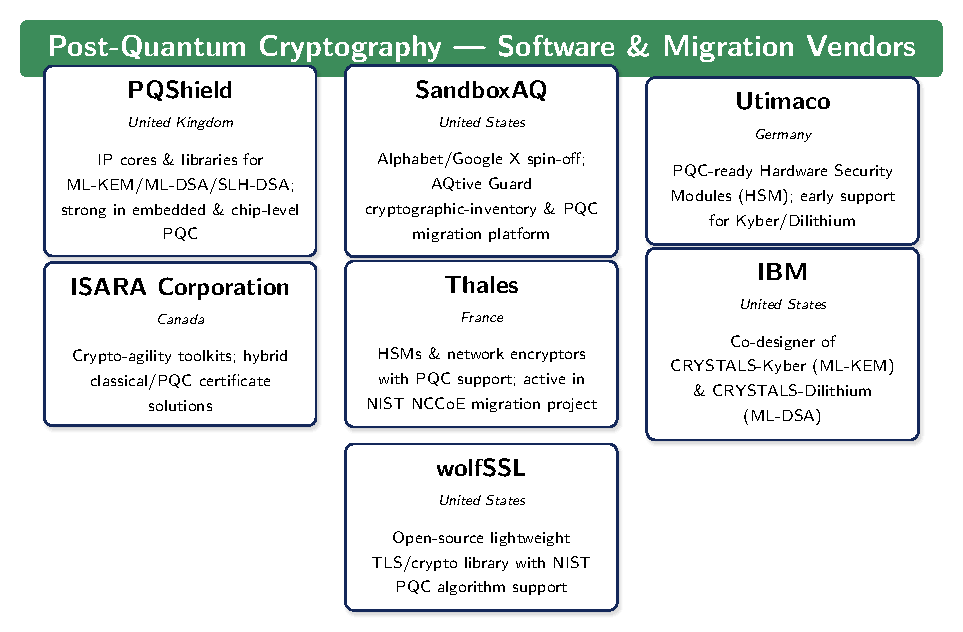
\includegraphics[width=0.98\linewidth]{figs/fig_pqc_vendors.pdf}
% TODO: لوگو -- نام‌های پیشنهادی فایل در figs/logos/README.txt
% \vspace{4pt}
% \includegraphics[height=1.1cm]{figs/logos/pqshield.png}\hfill
% \includegraphics[height=1.1cm]{figs/logos/sandboxaq.png}\hfill
% \includegraphics[height=1.1cm]{figs/logos/ibm.png}
\caption{شرکت‌های فعال در توسعهٔ نرم‌افزار و سخت‌افزار رمزنگاری پساکوانتومی \Cite{tqi2026pqccompanies,pqshield2026,nccoe2024migration}}
\label{fig:pqcvendors}
\end{figure}

شایان ذکر است که دو الگوریتم اصلی استانداردشدهٔ \lr{NIST} -- یعنی \lr{ML-KEM} و \lr{ML-DSA} -- به‌ترتیب از طرح‌های \lr{CRYSTALS-Kyber} و \lr{CRYSTALS-Dilithium} مشتق شده‌اند که با مشارکت مستقیم پژوهشگران \lr{IBM} طراحی شده بودند؛ این نکته نشان می‌دهد که مرز میان «استاندارد دولتی» و «محصول صنعتی» در حوزهٔ \lr{PQC} بسیار کم‌رنگ است و بومی‌سازی این فناوری می‌تواند از همان کتابخانه‌های متن‌باز (مانند \lr{liboqs} یا \lr{wolfSSL}) آغاز شود.

%=====================================================================
